\chapter{Working with Binary-Valued Graph Signals} % Main chapter title

\label{chap:binary} 

\lhead{Chapter 7. \emph{Working with Binary-Valued Graph Signals}} 

So far in this thesis, we have focused on reconstruction and regression models for real-valued graph signals, as discussed in \cref{chap:gsr_2d,chap:kgr_rnc_2d,chap:nd_gsp,chap:variance}. In this chapter, we shift our attention to scenarios where the signal of interest is binary-valued. Such signals can be employed to describe node classification tasks conducted over networks. For instance, consider the task of predicting whether users in a social network will click on a specific online advertisement. It is reasonable to assume that closely connected individuals within the network are more likely to have a similar probability of clicking than distantly connected individuals. Consequently, integrating this relational information into a predictive task may enhance accuracy. In this example, the classification task is binary as visualised in \cref{fig:binary_class_graph}. However, there may also be situations in which each node must be classified into one of many groups. In this case, we have a multiclass classification, as visualised in \cref{fig:mutliclass_graph}. \cite{Li2012}


\begin{figure}[t] 
    \begin{center}
        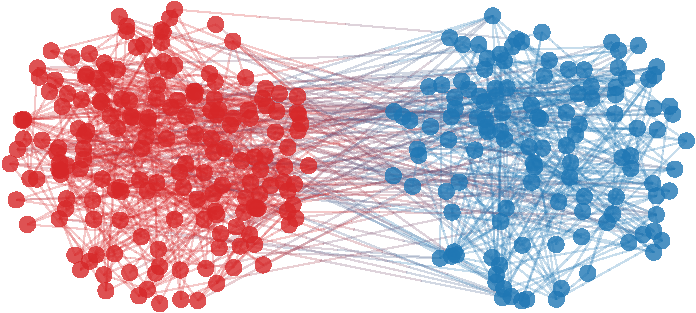
\includegraphics[width=0.8\linewidth]{Figures/2class_graph.pdf}
    \end{center}
   \caption[Visualisation of a binary classification task over a network]{An example visualisation of a binary classification task over a network.} 
    \label{fig:binary_class_graph}
\end{figure} 

\begin{figure}[t] 
    \begin{center}
        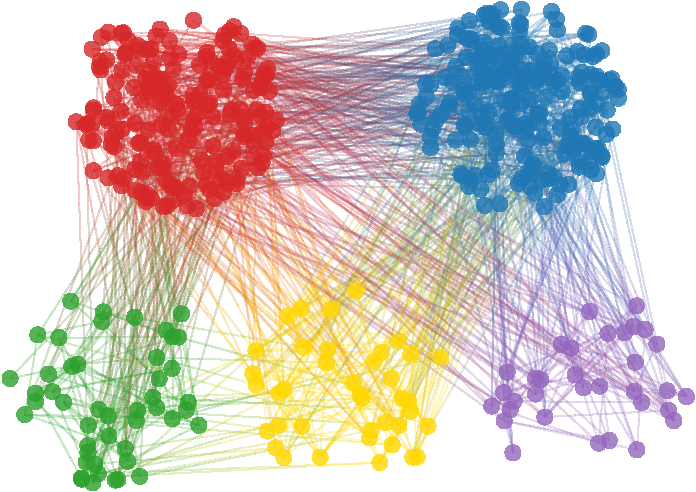
\includegraphics[width=0.8\linewidth]{Figures/multiclass_graph.pdf}
    \end{center}
   \caption[Visualisation of a multiclass classification task over a network]{An example visualisation of a multiclass classification task over a network.} 
    \label{fig:mutliclass_graph}
\end{figure} 



\section{Logistic Graph Signal Reconstruction}

\label{sec:lgsr}



Consider a binary signal reconstruction problem over a Cartesian product graph of order $d$. The observed graph signal, $\Yt$, is an order-$d$ tensor of shape $(N_1, N_2, .., N_d)$, with binary-valued elements. This is accompanied by another binary tensor, $\St$, of the same shape. As in previous chapters, $\St$ contains the information about which elements of $\Yt$ were observed by holding ones at elements where successful observations were made and zeros elsewhere. The goal is to predict the value of the graph signal at elements where no observation was made. 

\begin{equation*}
    \text{input data} = \Big\{\; \Yt \in \{0, 1\}^{N_1 \times ... \times N_d}, \;\; \St \in \{0, 1\}^{N_1 \times ... \times N_d} , \;\; \A \in \R^{N \times N} \; \Big\}
\end{equation*}

In the following, we assume each observed element, $\nn$, of the tensor, $\Yt$, follows a Bernoulli distribution with a mean $\Mt_\nn$. All other elements of $\Yt$ not in the set of observed elements $\mathcal{S}$ are zero with probability one. 

\begin{equation}
    \Yt_\nn \sim  \begin{cases}
        \text{Bern}\left(\Mt_\nn \right) & \text{if} \;\; \nn \in \mathcal{S} \\
        \text{Bern}\left(0\right) & \text{otherwise}
    \end{cases}
\end{equation}


$\Mt$ is the mean tensor, which has the same shape as $\Yt$ and elements falling within the interval $[0, 1]$. For a given mean, $\Mt$, the probability of observing a binary signal $\Yt$ is therefore given by 

\begin{equation}
    p(\Yt \, | \, \Mt) = \prod_{\nn \in \mathcal{S}} \Mt_\nn^{\Yt_\nn}\left(1 - \Mt_\nn\right)^{1 - \Yt_\nn}
\end{equation}

As such, the log-likelihood of observing a signal $\Yt$ is given by 

\begin{equation}
   \log p(\Yt \, | \, \Mt) = \s^\top \big(\y \circ \log \muu + \left(\one  - \y\right) \circ \log \left(\one - \muu \right)\big)
\end{equation}

where $\s = \vecrm{\St}, \; \y = \vecrm{\Yt}$ and $\muu = \vecrm{\Mt}$. Here, the logarithm function is understood as being applied element-wise.

As in previous chapters, we would like to encode the belief that the underlying signal, in this case $\Mt$, is smooth with respect to the topology of the graph. However, since its elements fall within the interval $[0, 1]$, we need a function that enforces this restriction. As with standard logistic regression (see, for example \cite{Murphy2012}), this can be achieved by appling a logistic link (sigmoid) function. In the following, we assume that the mean tensor, $\Mt$, is generated by applying this function to a real-valued tensor graph signal $\Ft \in \R^{N_1 \times ... \times N_d}$. 

\begin{equation}
    \label{eq:logistic_link}
    \Mt(\Ft) = \frac{1}{1 + \exp(-\Ft)} \quad \Longleftrightarrow \quad \muu(\f) = \frac{1}{1 + \exp(-\f)}
\end{equation}

As in previous chapters, we make the assumption that $\f = \vecrm{\Ft}$ is smooth with respect to the topology of the graph by assigning it the following prior. 

\begin{equation}
    \f  \, \sim \, \mathcal{N}\left( \zero, \, \gamma^{-1} \HH^2 \right) 
\end{equation}

where $\HH = \U \D_\Gt \U^\top$ is a graph filter constructed by applying a filter function $g(\cdot)$ to the graph Laplacian. By applying this assumption to $\Ft$, it is also applied by proxy to the mean tensor $\Mt$. \Cref{fig:logistic_gsr} gives some visual intuition for this by showing a colour-map of a smooth signal $\Ft$ existing over a 2D lattice graph, along with the corresponding mean $\Mt$. 

\begin{figure}[t] 
    \begin{center}
        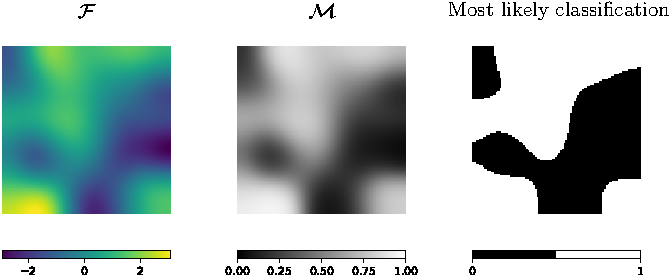
\includegraphics[width=\linewidth]{Figures/logistic_gsr.pdf}
    \end{center}
   \caption[Visualisation of a smooth graph signal and corresponding Bernoulli mean]{An example visualisation of a random smooth graph signal $\Ft$, and the corresponding mean signal $\Mt$ found by applying the logistic link function given in \cref{eq:logistic_link}. On the right, we show the most likely observed graph signal $\Yt$ for this mean, which is the binary signal given by $\Mt > 0.5$. The underlying graph in this case is a $100 \times 100$ grid of lattice points. } 
    \label{fig:logistic_gsr}
\end{figure} 

Through the application of Bayes' rule, we can derive an equation for the posterior distribution of $\Ft$ given $\Yt$. The Maximum A Posteriori (MAP) estimator for $\Ft$ corresponds to the value that minimizes the negative log-likelihood of this distribution. Thus, we introduce the objective function $\xi(\f) $, which is equal to $ -\log p(\f \, | \, \y)$ up to an additive constant.
 
\begin{equation*}
    \xi(\f) = -\s^\top \big(\y \circ \log \muu(\f) + \left(\one  - \y\right) \circ \log \left(\one - \muu(\f) \right)\big) + \frac{\gamma}{2} \f^\top \HH^{-2} \f
\end{equation*}

Unlike the normal models of the previous sections, no closed-form solution exists to minimise this expression. A standard approach to solving optimisation problems of this form is to use the Iteratively Reweighted Least Squares (IRLS) algorithm. IRLS algorithms have been independently discovered several times and have been studied for over 50 years. Their main use today is found in $L^p$ norm optimisation problems such as sparse recovery (e.g. \cite{Gorodnitsky1997,Daubechies2010}) and maximum likelihood estimation within a generalized linear models \citep{Nelder1972}. 

The IRLS algorithm begins with an initial estimate $\f_0$, which is then iteratively refined to reach the global minimum. Each step is given by the following update formula. 

\begin{equation}
    \f_{k+1} = \f_{k} - \PP^{-1} \g(\f)
\end{equation}

where $ \g(\f) = \nabla \xi(\f) \in \R^N$ is the gradient of the optimisation objective $\xi(\f)$ with respect to the vector $\f$, and $\PP = \nabla^2 \xi(\f) \in \R^{N \times N}$ is the Hessian, which is the matrix of second derivatives. In our case, the gradient is given by 

\begin{equation}
    \g(\f) = \frac{\partial \xi(\f)}{\partial \f} = \D_\St \big(\muu(\f) - \y\big) + \gamma \HH^{-2} \f
\end{equation}

and the Hessian is given by 

\begin{equation}
    \PP(\f) = \frac{\partial \g(\f)}{\partial \f} =  \D_{\muu}(\f) + \gamma \HH^{-2}
\end{equation}

where $\D_{\muu}(\f)$ is a diagonal matrix with the following definition. 

\begin{equation*}
    \D_{\muu}(\f) = \text{diag}\big(\s \circ \muu(\f) \circ (\one - \muu(\f))\big)
\end{equation*}

A derivation of the expressions for both gradient and the Hessian can be found in \cref{the:gradient_and_hesian}. Note that they are both a function of $\f$. 


\section{Logistic Kernel Graph Regression} 

 
\label{sec:lkgr}


\section{Logistic Regression with Network Cohesion}

\label{sec:lrnc}

\section{Multiclass Methods}

\label{sec:multiclass}


\section{Approximate Sampling via the Laplace Approximation}

\label{sec:lsamp}

